\chapter{提案}
\label{chap:teian}

%ーーーーーーーーーーーーーーーーーーーーーーーーーーーー

\section{概要}
本研究で提案している手法の流れを下記に示す. 

\begin{enumerate}
  \item GooglePlayとXに投稿されたアプリレビューをスクレイピングして取得, 前処理
  \item レビュー文に含まれるバグレポートやアプリに対する要望を示す箇所を自動抽出
  \item 抽出結果を利用しクラスタリング
  \item 分析された結果をwebブラウザ上に可視化
\end{enumerate}

提案手法の流れを図\ref{fig:nagare}に示す. 

\begin{figure}[hbtp]
  \centering
  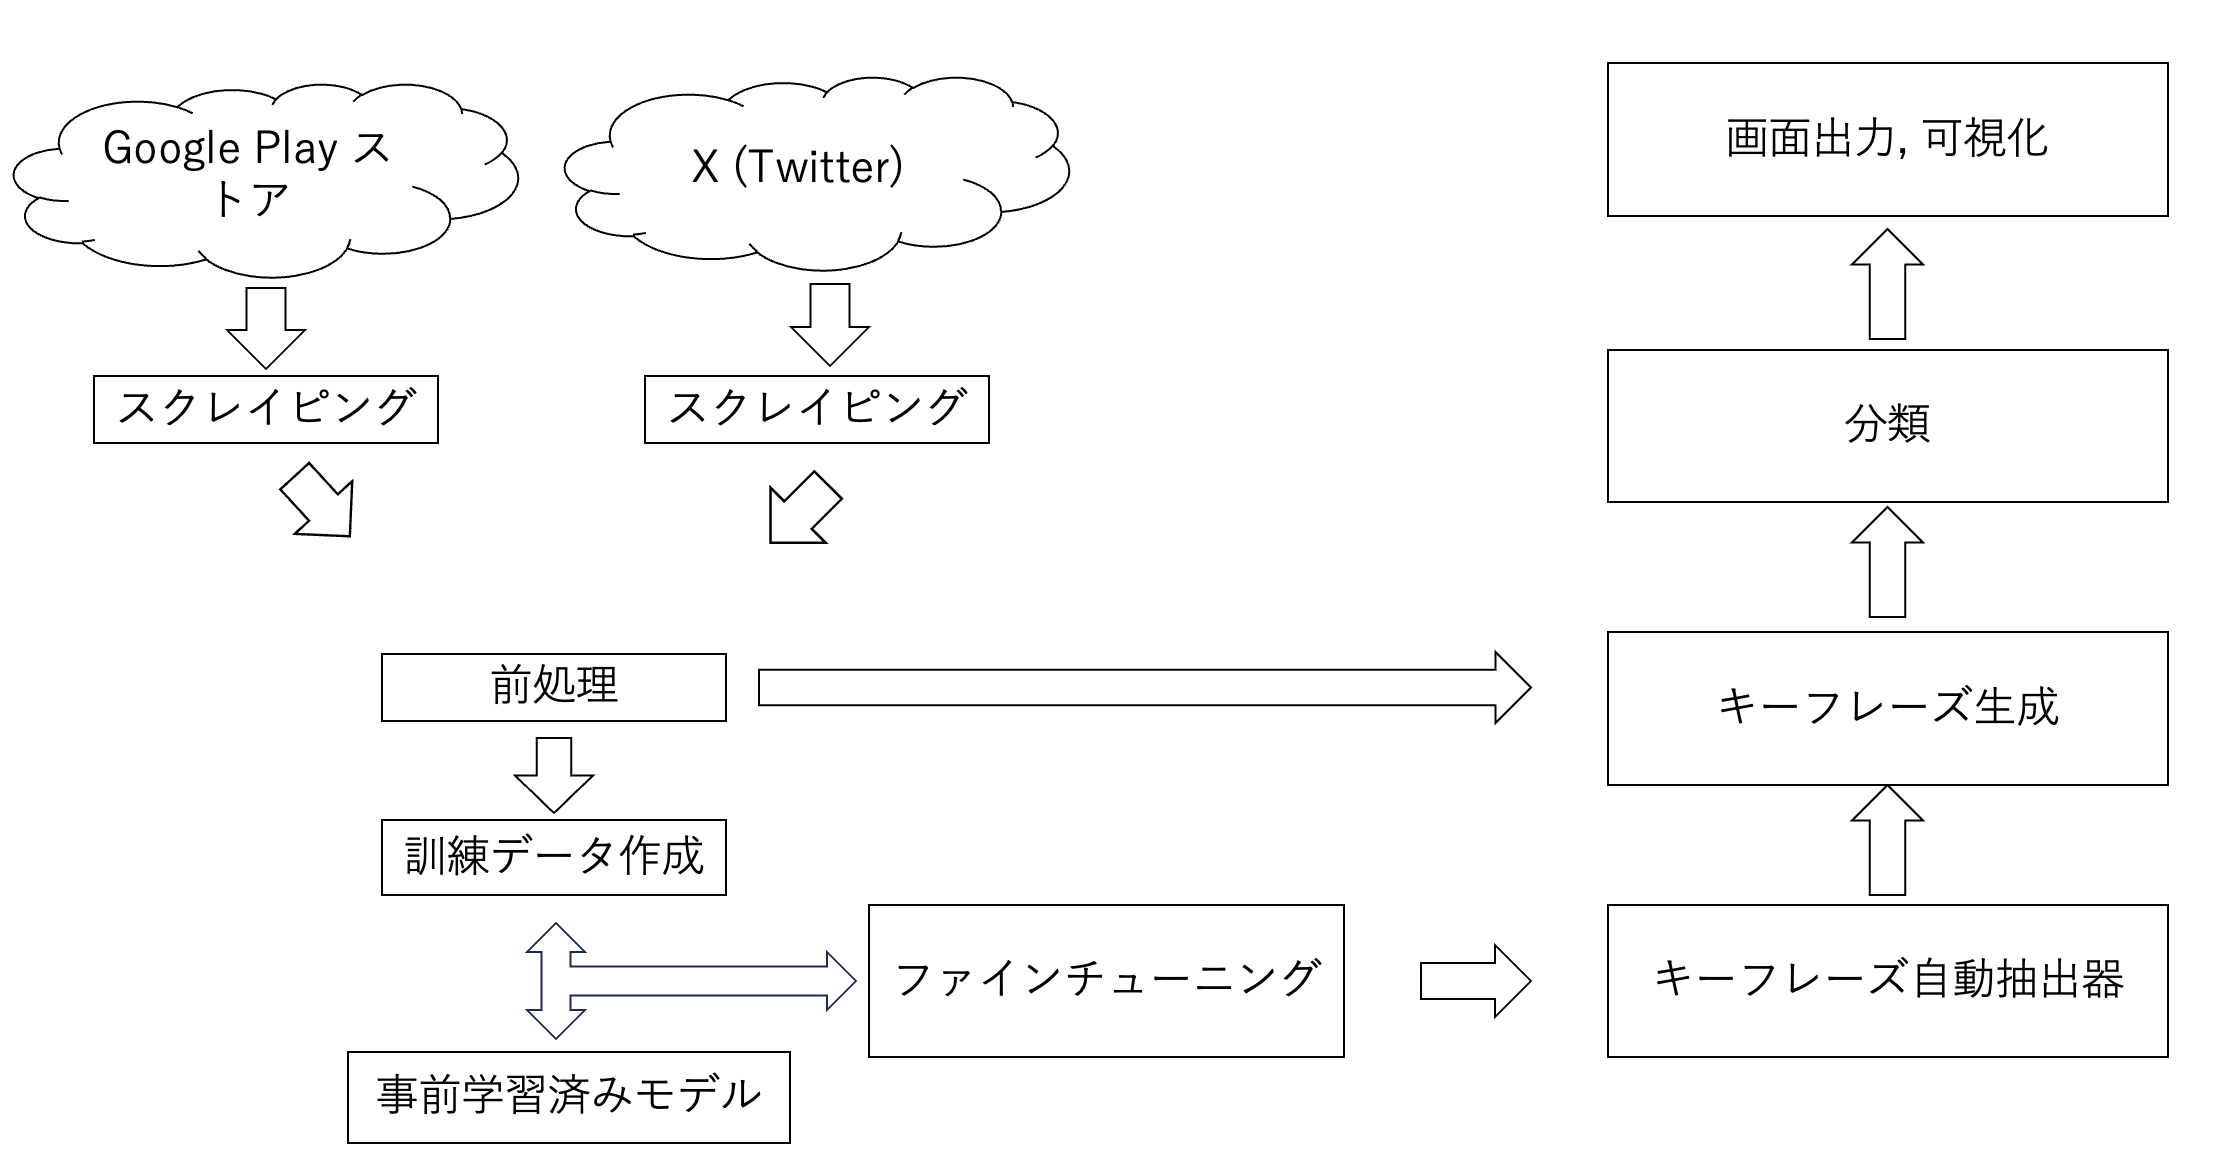
\includegraphics[width=\linewidth]
       {contents/images/zisso_nagare.png}
  \caption{実装した提案手法の流れ\label{fig:nagare}}
\end{figure}

%ーーーーーーーーーーーーーーーーーーーーーーーーーーーー

\section{対象アプリとレビュー}
本研究では川面による先行研究\cite{kawatsura}のデータセットを使用するため対象アプリは先行研究のアプリに合わせている. 注意点として, BuzzVideoは2022年3月をもってサービスを終了しているため現在は収集対象のアプリには含まれない. そのため, 本研究で新たに取得するレビューの対象となるアプリはBuzzVideo以外の12のアプリである. 
対象となっているアプリを表\ref{tb:taisyouapuri}に示す. 
\begin{table}[htbp]
  \caption{本研究の対象アプリ一覧}
  \label{tb:taisyouapuri}
  \begin{center}
  \begin{tabularx}{\linewidth}{X|l|X}
    \hline
    \mbox{アプリ名}\mbox{(一部略称)}&\mbox{Google Playストアの}\mbox{パッケージID}&\mbox{Twitterの}\mbox{検索キーワード}\\\hline\hline
    にゃんトーク&com.akvelon.meowtalk&にゃんトーク\\\hline
    スマートニュース&jp.gocro.smartnews.android&スマートニュース\\\hline
    PayPay&jp.ne.paypay.android.app&paypay\\\hline
    Coke ON&com.coke.cokeon&coke on\\\hline
    Google Fit&com.google.android.apps.fitness&google fit\\\hline
    Simeji&com.adamrocker.android.input.simeji&simeji\\\hline
    Lemon8&com.bd.nproject&lemon8\\\hline
    楽天ペイ&jp.co.rakuten.pay&楽天ペイ\\\hline
    majica&com.donki.majica&majica\\\hline
    LINE MUSIC&jp.linecorp.linemusic.android&line music\\\hline
    BuzzVideo&com.ss.android.article.topbuzzvideo&buzzvideo\\\hline
    ファミペイ&jp.co.family.familymart\verb|_|app&ファミペイ\\\hline
    CapCut&com.lemon.lvoverseas&capcut\\\hline
  \end{tabularx}\end{center}
\end{table}

%ーーーーーーーーーーーーーーーーーーーーーーーーーーーー

\section{事前準備}
本研究で対象としているアプリに関するGooglePlayストアのレビュー及びポスト(ツイート)をスクレイピングし, 分析対象となるデータセットを作成する. 本研究にて使用するデータセットは先行研究によって作成された13個のアプリレビューのデータセットに加え, 本研究で新たに収集したアプリレビューのデータセットを使用する. 対象アプリを先行研究に合わせた理由としては, 現在, Xのポストの収集可能な数に制限がある影響で十分な数のポストが収集できなかったためである. Xのポスト取得数の制限に関しては\ref{sec:x}で詳しく述べる. 
そして, スクレイピングしたデータから有用な箇所を自動抽出するために一般的な自然言語処理で行われる前処理を行う. 

%ーーーーーーーーーーーーーーーーーーーーーーーーーーーー

\section{自動抽出}
スクレイピングして前処理された大量の文章から開発に有用な文章を絞り込み, かつその文章の中からバグの報告やアプリに対する要望に関して記述している部分を自動抽出する. これにより自動的に開発に有用なレビューかどうかを取捨選択されつつ, 有用なレビューである場合にはその文章の中に含まれるバグの報告やアプリに対する要望に関して記述している部分を抽出できる. 自動抽出のために日本語のデータで事前学習済みの言語表現モデルである日本語BERTに対して質問応答形式のfune-tuningを行うことで自動抽出器を生成する. 
抽出を行う文章の特徴をモデルに理解させるために質問文にその文章がGooglePlayストアのレビューなのかXの文章なのかという「カテゴリー」の情報と「アプリ名」という2つの情報を加えることにより学習性能を上げる. 図\ref{fig:fine-tuning}に質問応答形式によるfine-tuningのモデルを示す. 

\begin{figure}[hbtp]
  \centering
  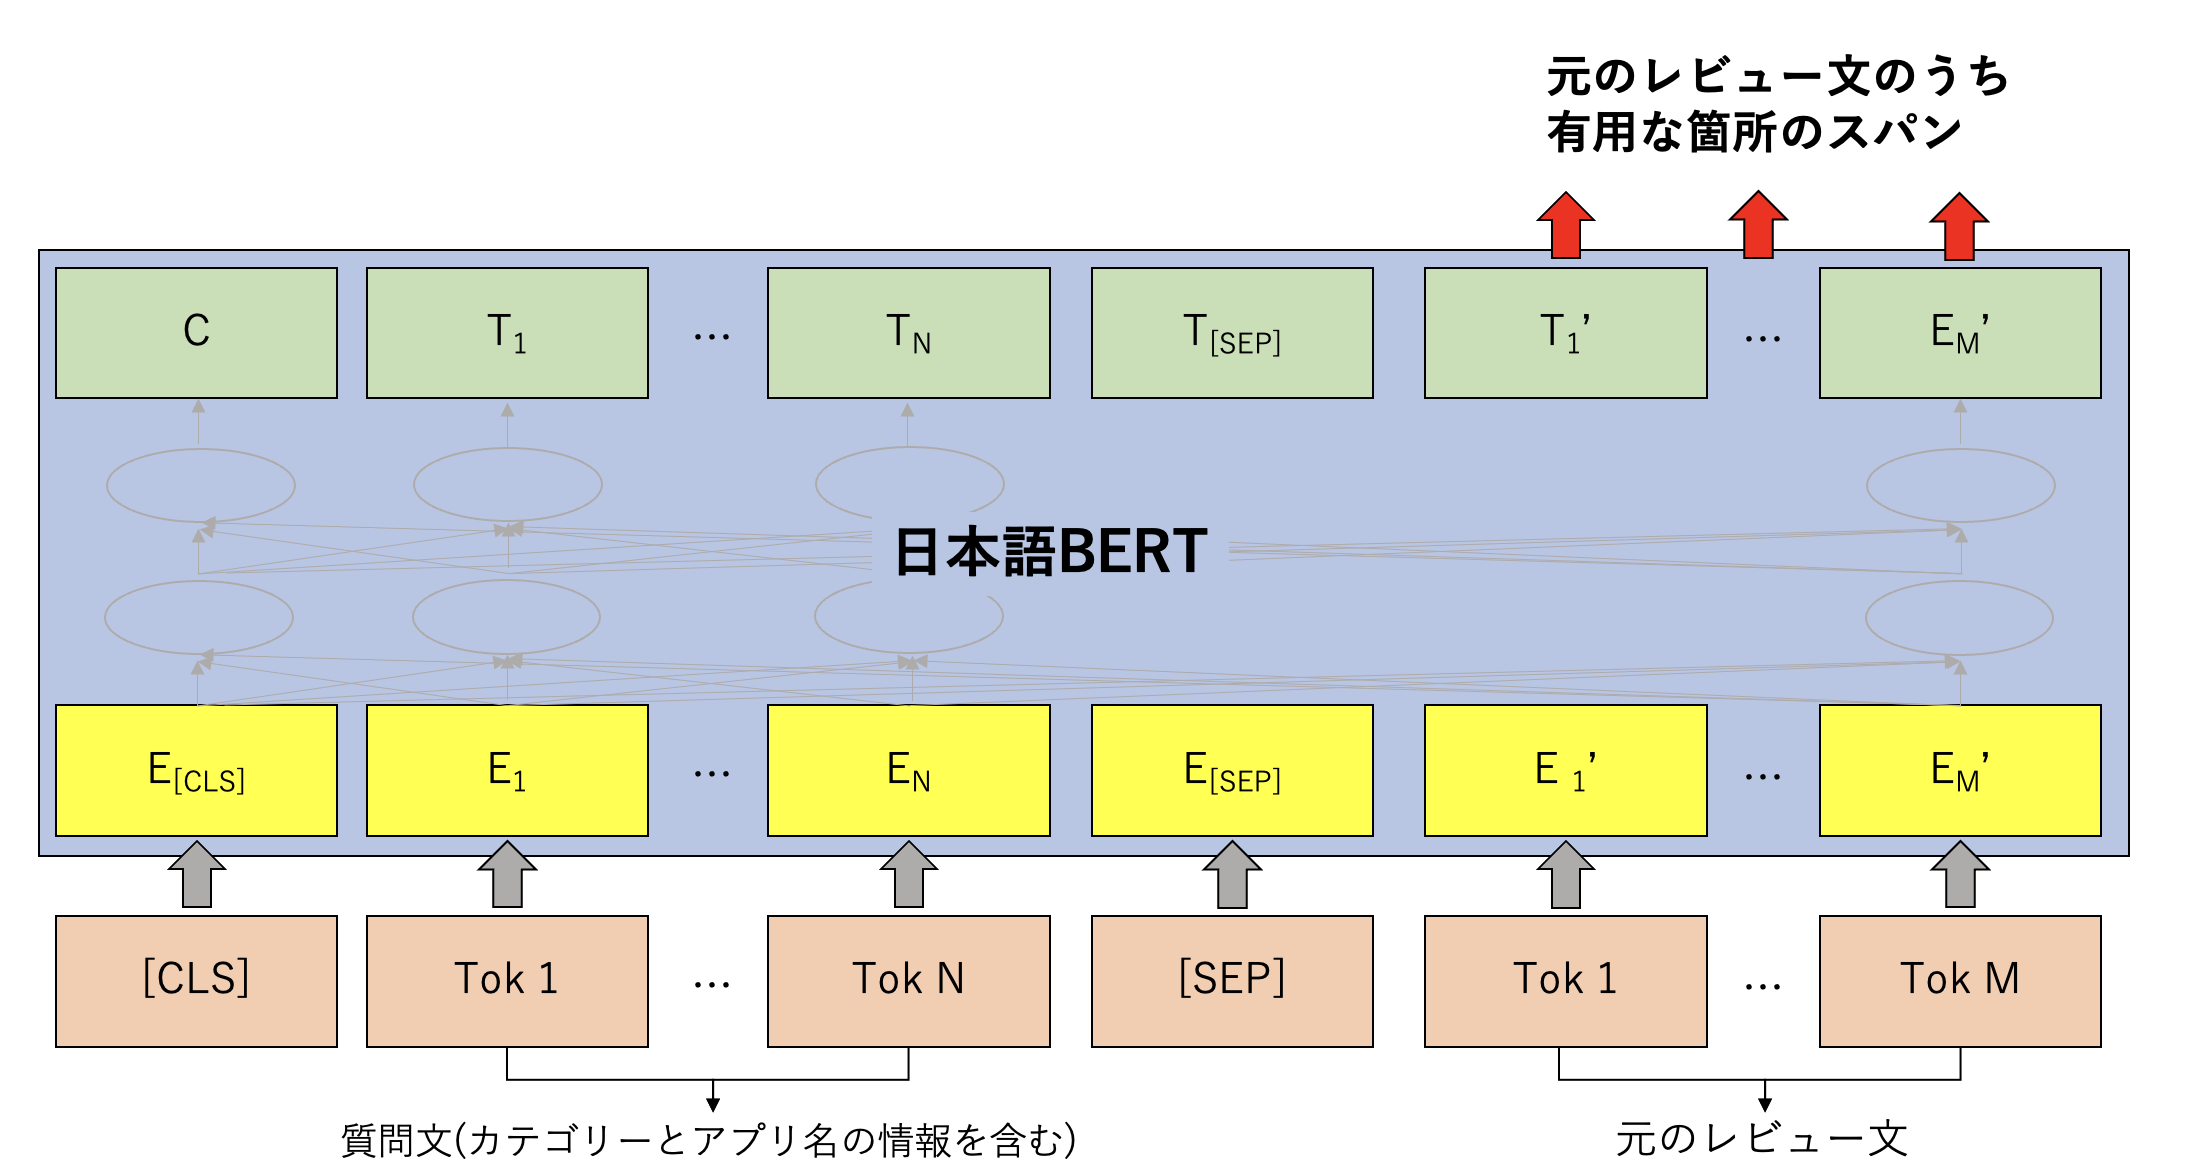
\includegraphics[scale=0.3]
       {contents/images/fine-tuning.png}
  \caption{ファインチューニング\label{fig:fine-tuning}}
 \end{figure}

また, 図\ref{fig:answer}に質問文とその答えの例を示す. 質問文にアプリの欠陥やアプリに対する要望を尋ねる文章を与え, その答えとして欠陥や要望を示す箇所を返すようにしている. 
\begin{figure}[hbtp]
  \centering
  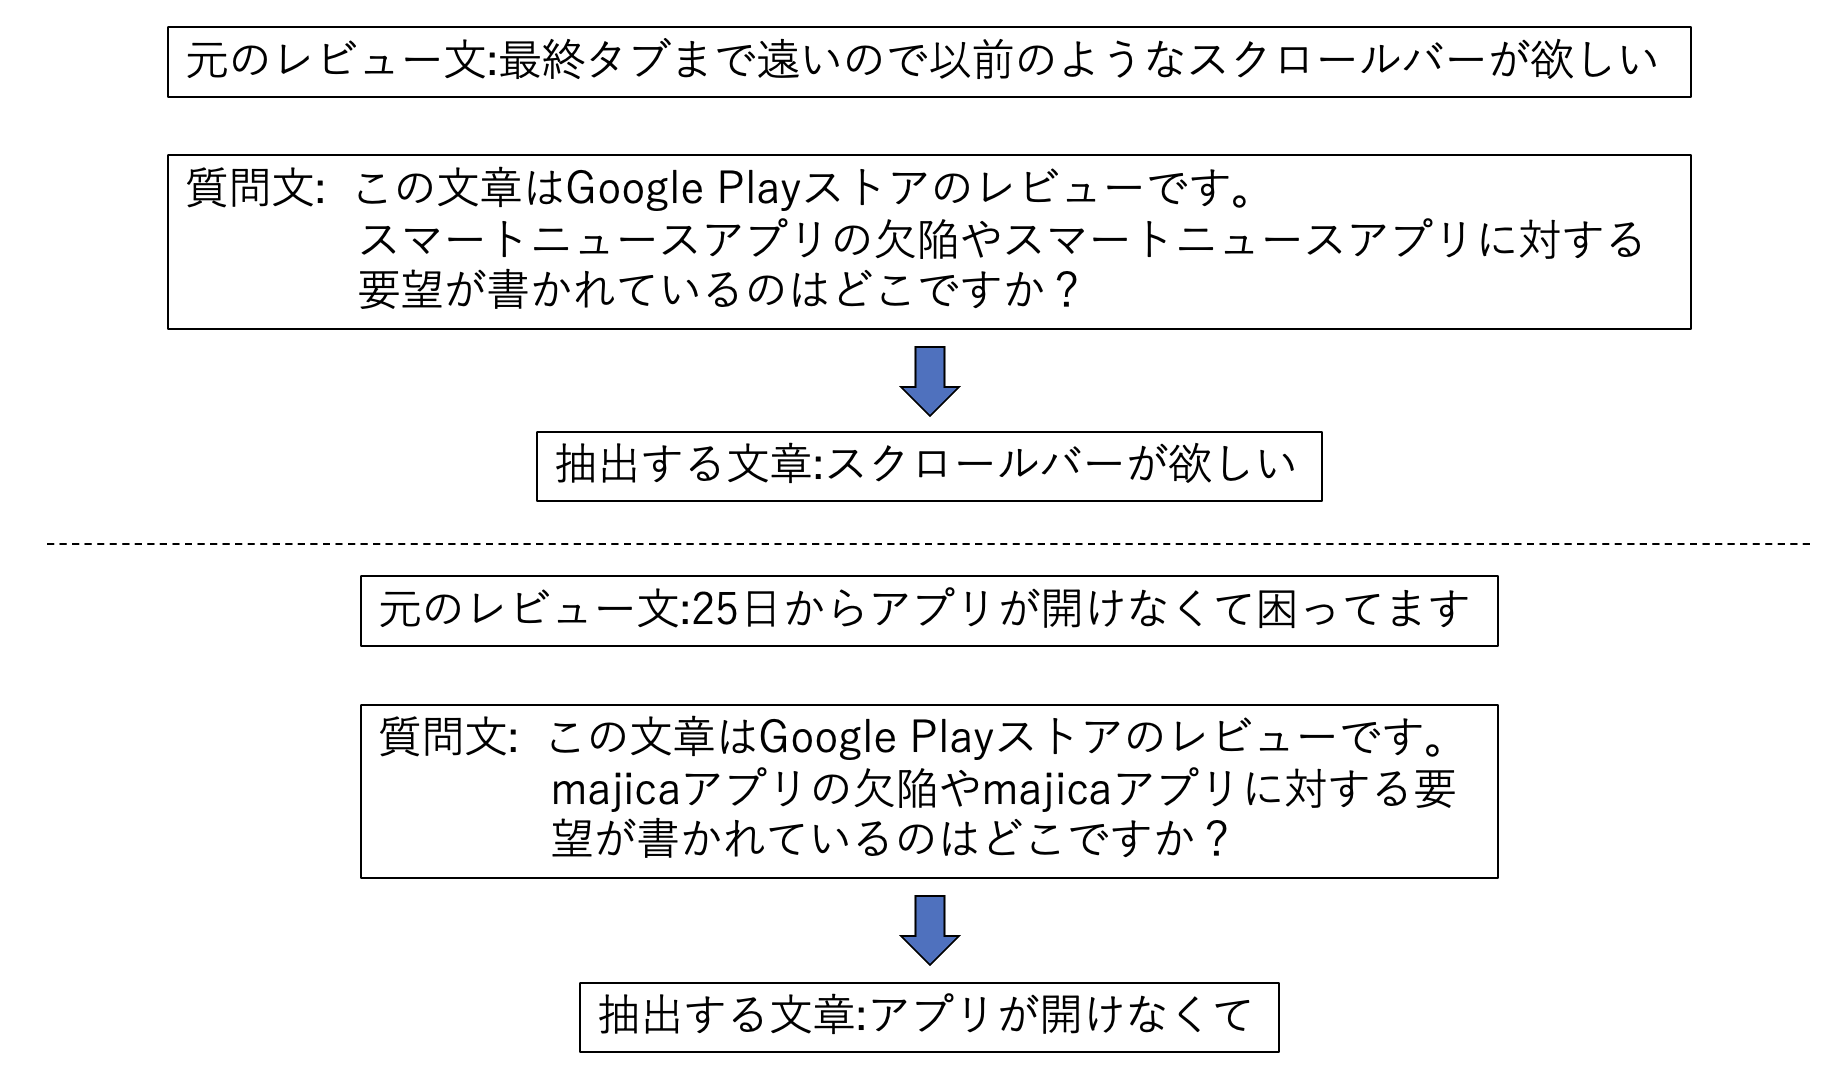
\includegraphics[scale=0.4]
       {contents/images/answer.png}
  \caption{有用な箇所の抽出例\label{fig:answer}}
\end{figure}

%ーーーーーーーーーーーーーーーーーーーーーーーーーーーー

\section{クラスタリング}
抽出した文章のクラスタリングには既存研究のクラスタリング手法\cite{sira}を参考にして実装する. 参考にした既存研究の手法は以下の3つの手順を踏んでいる. 
\begin{enumerate}
  \item Universal Sentence Encoder (USE)を用いて, 問題のある特徴語句を512次元のベクトルに変換
  \item 重み付き無向グラフを構成し, 各問題機能をノードとし, 2つの問題機能のUSEベクトル間のコサイン類似度スコア(比率)をノード間の重みとする. 比率は入力ハイパーパラメータであり, 問題のある機能間の意味的相関を測定. 
  \item このグラフに対して, Chinese Whispers (CW)を実行し, 問題のある特徴量をクラスタリング
\end{enumerate}

既存研究では英語の文章をベクトルに変換するためにUniversal Sentence Encoder (USE)を使用しているが, 今回は対象が日本語の文章であるため, Sentence-BERTの日本語モデルを使用する. Sentence-BERT\cite{sentence-bert}とは, 事前学習されたBERTモデルとSiamese Networkを使い, 高品質な文ベクトルを作る手法である. このモデルを使用することで, 高品質な文ベクトルが作成できる. 
したがって本研究でのクラスタリング手法は下記である. 
\begin{enumerate}
  \item Sentence-BERTの日本語モデルを用いて, 抽出した文章をベクトルに変換
  \item 重み付き無向グラフを構成し, 抽出した文章をノードとし, 2つの抽出した文章間のベクトル間のコサイン類似度スコア(比率)をノード間の重みとする. 比率は入力ハイパーパラメータであり, 抽出した文章間の意味的相関を測定. 
  \item このグラフに対して, Chinese Whispers (CW)を実行し, 問題のある特徴量をクラスタリング
\end{enumerate}

%ーーーーーーーーーーーーーーーーーーーーーーーーーーーー

\section{画面出力・可視化}
分類した結果を用いて画面出力を行う. 開発者がアプリの修正やアップデートを行った後でユーザがどのようなレビューを挙げているか, 特定の機能に関するユーザレビューを絞り込むことができれば開発をサポートできると考えた. したがって, レビューが投稿された期間やレビュー文のキーワードで絞り込み検索することが可能なツールを作成した. そして, 日ごとのレビュー数を表す折れ線グラフとクラスタに含まれるレビュー数の上位10個を表す棒グラフを作成した. この2つのグラフは検索結果に応じて動的に変化するようになっている. 
このような機能をwebアプリとして実装することにより, 開発者がレビューを理解, 分析しやすいように可視化されている. 